\renewcommand*{\arraystretch}{1.1}

\label{sec:bi-read-18}
\noindent\begin{tabularx}{\queryCardWidth}{|>{\queryPropertyCell}c|X|}
	\hline
	query & BI / read / 18 \\ \hline
%
	title & How many persons have a given number of posts \\ \hline
%
    pattern & \hfill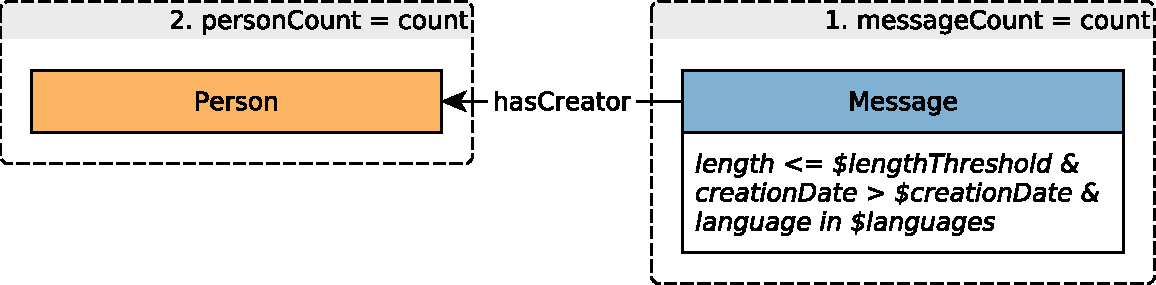
\includegraphics[scale=\patternscale,margin=0cm .2cm]{patterns/bi-read-18}\hfill\vadjust{} \\ \hline
%
	desc. & For each Person, count the number of Messages (Posts \& Comments) they
made.

Only consider messages with:

\begin{itemize}
\tightlist
\item
  length below the \texttt{lengthThreshold}
\item
  creationDate after \texttt{creationDate} (TODO - is after exclusive or
  inclusive, does it allow equality?)
\item
  any of the given \texttt{languages} (TODO - only Posts have a
  language, messages do not)
\end{itemize}
 \\ \hline
%
	
        group by &
        \multicolumn{1}{>{\raggedright}X|}{
            \varNameText messageCount
            } \\ \hline
	
%
    
        params &
        \innerCardVSpace{\begin{tabularx}{\attributeCardWidth}{|>{\paramNumberCell}c|>{\varNameCell}M|>{\typeCell}m{\typeWidth}|Y|} \hline
        \cellcolor{parameter} \color{white} \footnotesize $\mathsf{1}$ &creationDate& Date &  \\ \hline
        \cellcolor{parameter} \color{white} \footnotesize $\mathsf{2}$ &lengthThreshold& TODO (32-bit Integer?) &  \\ \hline
        \end{tabularx}}\innerCardVSpace \\ \hline
	
%
	
        result &
        \innerCardVSpace{\begin{tabularx}{\attributeCardWidth}{|>{\resultNumberCell}c|>{\varNameCell}M|>{\typeCell}m{\typeWidth}|>{\resultOriginCell}c|Y|} \hline
        $\mathsf{1}$ & messageCount & 32-bit Integer &A&
                number of messages created \\ \hline
        $\mathsf{2}$ & personCount & 32-bit Integer &A&
                the number of Persons with `messageCount` messages \\ \hline
        \end{tabularx}}\innerCardVSpace \\ \hline
	
%
	sort        &
        \innerCardVSpace{\begin{tabular}{|>{\sortNumberCell}c|>{\varNameCell}l|>{\directionCell}c|} \hline
        $\mathsf{1}$ & personCount & $\desc$ \\ \hline
        \end{tabular}}\innerCardVSpace \\ \hline
	%
	%
	CPs &
	\multicolumn{1}{>{\raggedright}l|}{
	    \chokePoint{1.1}, 
	    \chokePoint{1.2}, 
	    \chokePoint{1.6}, 
	    \chokePoint{3.2}, 
	    \chokePoint{4.2}, 
	    \chokePoint{4.3}
	    } \\ \hline
	%
    %
\end{tabularx}
\queryCardVSpace